\section*{سوال ۴}

شکل زیر را در نظر بگیرید:  

\begin{figure}[H]
    \centering
    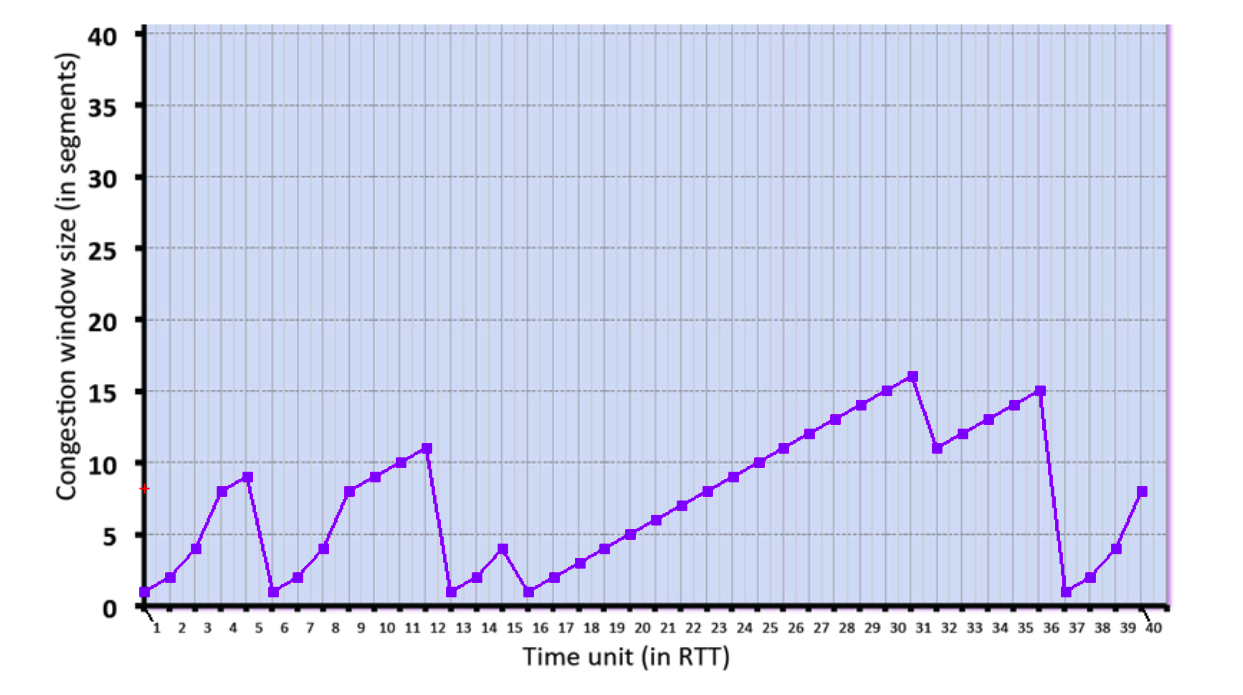
\includegraphics[width=0.95\textwidth]{Questions/pics/Q4.png}
    \caption{}
    \label{fig:small-example}
\end{figure}

این شکل تغییرات اندازه‌ی پنجره‌ی ازدحام (\lr{congestion window}) در پروتکل \lr{TCP} را در ابتدای هر واحد زمانی نشان می‌دهد (هر واحد زمان برابر با یک \lr{RTT} است).  
در مدل انتزاعی این مسئله فرض می‌شود که \lr{TCP} در ابتدای هر واحد زمانی، یک پنجره کامل از بسته‌ها (\lr{flight}) به اندازه‌ی مقدار \lr{cwnd} ارسال می‌کند.  

نتیجه‌ی ارسال این مجموعه از بسته‌ها می‌تواند یکی از حالت‌های زیر باشد:
\begin{itemize}
    \item همه‌ی بسته‌ها در پایان واحد زمانی تأیید (\lr{ACK}) می‌شوند.
    \item برای اولین بسته، انقضای زمان (\lr{timeout}) رخ می‌دهد.
    \item برای اولین بسته، سه تأیید تکراری (\lr{triple duplicate ACK}) دریافت می‌شود.
\end{itemize}

در این مسئله خواسته شده است دنباله‌ی رویدادها (\lr{ACK}ها و از‌دست‌رفتن بسته‌ها) را بازسازی کنید که باعث تغییرات مشاهده‌شده در مقدار \lr{cwnd} در نمودار شده‌اند.  
مقدار اولیه‌ی \lr{cwnd = 1} و مقدار اولیه‌ی \lr{ssthresh = 8} (که با علامت + قرمز نشان داده شده است) در نظر گرفته می‌شود.

\begin{enumerate}[label=\alph*)]
    \item بازه‌های مربوط به \lr{slow start} را مشخص کنید.
    \item بازه‌های مربوط به \lr{congestion avoidance} را مشخص کنید.
    \item بازه‌های مربوط به \lr{fast recovery} را نشان دهید.
    \item در کدام لحظه(ها) \lr{timeout} رخ داده است؟
    \item در کدام لحظه‌(ها) \lr{triple duplicate ACK} رخ داده است؟
    \item در کدام لحظه‌ها مقدار \lr{ssthresh} تغییر کرده است؟
\end{enumerate}